\documentclass[a4paper]{article}
\usepackage[utf8]{inputenc}
\usepackage[english]{babel}
\usepackage{listings}
\usepackage[a4paper,margin=1.2in]{geometry}
\usepackage{indentfirst}
\usepackage{graphicx}
\usepackage{caption}
\usepackage{float}
\usepackage{hyperref}

\begin{document}

\title{Report: comparison of 9 global optimization methods on several test problems classes}
\author{Vladislav Sovrasov}
\date{}
\maketitle

\section{List of the algorithms}
\begin{itemize}
  \item Algorithm of global search (AGS) (\url{https://github.com/sovrasov/ags_nlp_solver})
  \item Multi Level Single Linkage (MLSL) (\url{https://nlopt.readthedocs.io/en/latest/NLopt_Algorithms/#mlsl-multi-level-single-linkage})
  \item DIRECT (\url{https://nlopt.readthedocs.io/en/latest/NLopt_Algorithms/#direct-and-direct-l})
  \item Locally-based DIRECT (DIRECT$l$) (\url{https://nlopt.readthedocs.io/en/latest/NLopt_Algorithms/#direct-and-direct-l})
  \item Dual Simulated Annealing (\url{https://github.com/sgubianpm/sdaopt})
  \item Differential Evolution (\url{https://docs.scipy.org/doc/scipy/reference/generated/scipy.optimize.differential_evolution.html#scipy.optimize.differential_evolution})
  \item Controlled Random Search (\url{https://nlopt.readthedocs.io/en/latest/NLopt_Algorithms/#controlled-random-search-crs-with-local-mutation})
  \item Simple (\url{https://github.com/chrisstroemel/Simple})
  \item StoGO (\url{https://nlopt.readthedocs.io/en/latest/NLopt_Algorithms/#stogo})
\end{itemize}

When conducting the comparison, the following parameters for the methods were employed:
\begin{itemize}
  \item in the AGS\(l\) method, the parameter of alternation the
global and local iterations was set to be equal to 5:1;
  \item in the DIRECT and DIRECT\(l\) methods, the parameter \(\epsilon=10^{-4}\);
  \item in the SDA method, the parameter \(visit=2.72\).
\end{itemize}

The rest parameters were varied subject to the problem class (see Table \ref{tab:params}).

\begin{table}
\begin{center}
\caption{Class-specific parameters of the optimization algorithms}
  \begin{tabular}{|l|{c}|{c}|{c}|}
    \hline
    & AGS, AGS\(l\) & CRS & DE\\
  \hline
  \(F_{GR}\) & \(r=3\) & popsize=150 & mutation=(1.1,1.9), popsize=60 \\
  \hline
  GKLS 2d Simple & \(r=4.6\) & popsize=200 & mutation=(1.1,1.9), popsize=60 \\
  \hline
  GKLS 2d Hard & \(r=6.5\) & popsize=400 & mutation=(1.1,1.9), popsize=60 \\
  \hline
  GKLS 3d Simple & \(r=3.7\) & popsize=1000 & mutation=(1.1,1.9), popsize=70 \\
  \hline
  GKLS 3d Hard & \(r=4.4\) & popsize=2000 & mutation=(1.1,1.9), popsize=80 \\
  \hline
  GKLS 4d Simple & \(r=4.7\) & popsize=8000 & mutation=(1.1,1.9), popsize=90 \\
  \hline
  GKLS 4d Hard & \(r=4.9\) & popsize=16000 & mutation=(1.1,1.9), popsize=100 \\
  \hline
  GKLS 5d Simple & \(r=4\) & popsize=25000 & mutation=(1.1,1.9), popsize=120 \\
  \hline
  GKLS 5d Hard & \(r=4\) & popsize=30000 & mutation=(1.1,1.9), popsize=140 \\
  \hline
\end{tabular}
  \label{tab:params}
\end{center}
\end{table}

\begin{table}
\begin{center}
\caption{Trials limits for the test problem classes}
  \begin{tabular}{|l|{c}|}
    \hline
  Problems class & Trials limit\\
  \hline
  \(F_{GR}\) & 5000 \\
  \hline
  GKLS 2d Simple & 8000 \\
  \hline
  GKLS 2d Hard & 9000 \\
  \hline
  GKLS 3d Simple & 15000 \\
  \hline
  GKLS 3d Hard & 25000 \\
  \hline
  GKLS 4d Simple & 150000 \\
  \hline
  GKLS 4d Hard & 250000 \\
  \hline
  GKLS 5d Simple & 350000 \\
  \hline
  GKLS 5d Hard & 600000 \\
  \hline
  \end{tabular}
  \label{tab:limits}
\end{center}
\end{table}

Since NLOpt hasn't an API to control parameters of the algorithms from Python, it was built with $\varepsilon=10^{-4}$ for DIRECT and DIRECT$l$ methods.

\section{List of the test problems}

\begin{itemize}
  \item Functions from $F_{GR}$ class. It consists of 100 multi-extremal problems of the same structure. The description can be found in \url{https://core.ac.uk/download/pdf/82313177.pdf}.
  \item Functions from classes generated by the GKLS generator (\url{http://wwwinfo.deis.unical.it/yaro/GKLS.html}).
\end{itemize}

Each class consists of 100 multi-extremal problems with 10 and more local minima. Problem is considered solved when optimization method placed a new trial point in the $\Delta$-vicinity of the known global optima $x^*$: $\Vert x^* - \widetilde{x} \Vert_{\inf} \le \Delta$.


\section{Results on the $F_{GR}$ class}

\begin{figure}[H]
  \center
  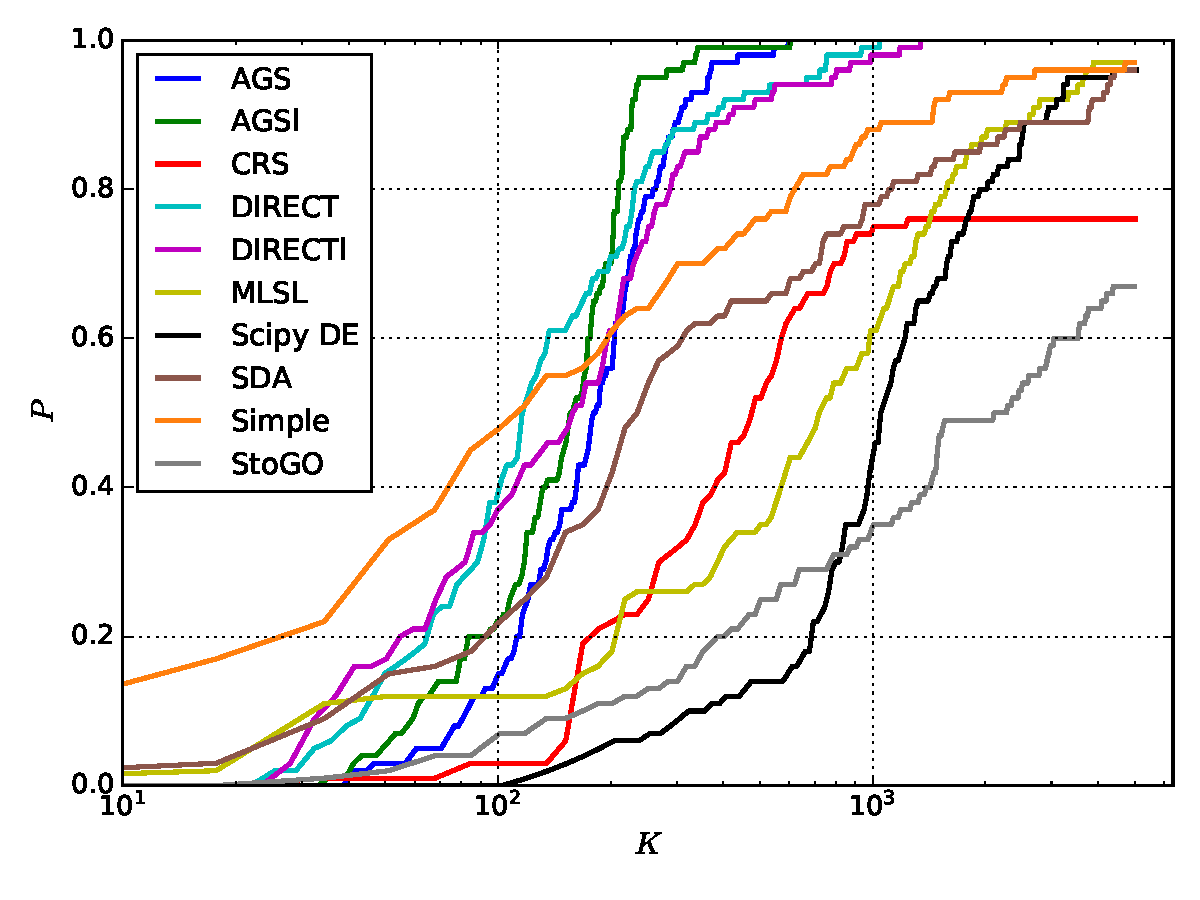
\includegraphics[width=0.95\textwidth]{../experiments/grish/cmc.pdf}
  \caption{$\Delta=10^{-2}$}
\end{figure}

%table grish
\begin{tabular}{lcc}
\hline
 Method   &  Average number of trials  &  Problems solved  \\
\hline
 AGS      &           193.11           &        100        \\
 AGSl     &           158.30           &        100        \\
 CRS      &           400.30           &        76         \\
 DIRECT   &           182.25           &        100        \\
 DIRECTl  &           214.92           &        100        \\
 MLSL     &           947.18           &        97         \\
 SDA      &           691.24           &        96         \\
 Scipy DE &          1257.34           &        96         \\
 Simple   &           374.12           &        97         \\
 StoGO    &          1336.78           &        67         \\
\hline
\end{tabular}
\section{Results on the $GKLS$ problems}

\begin{figure}[H]
  \center
  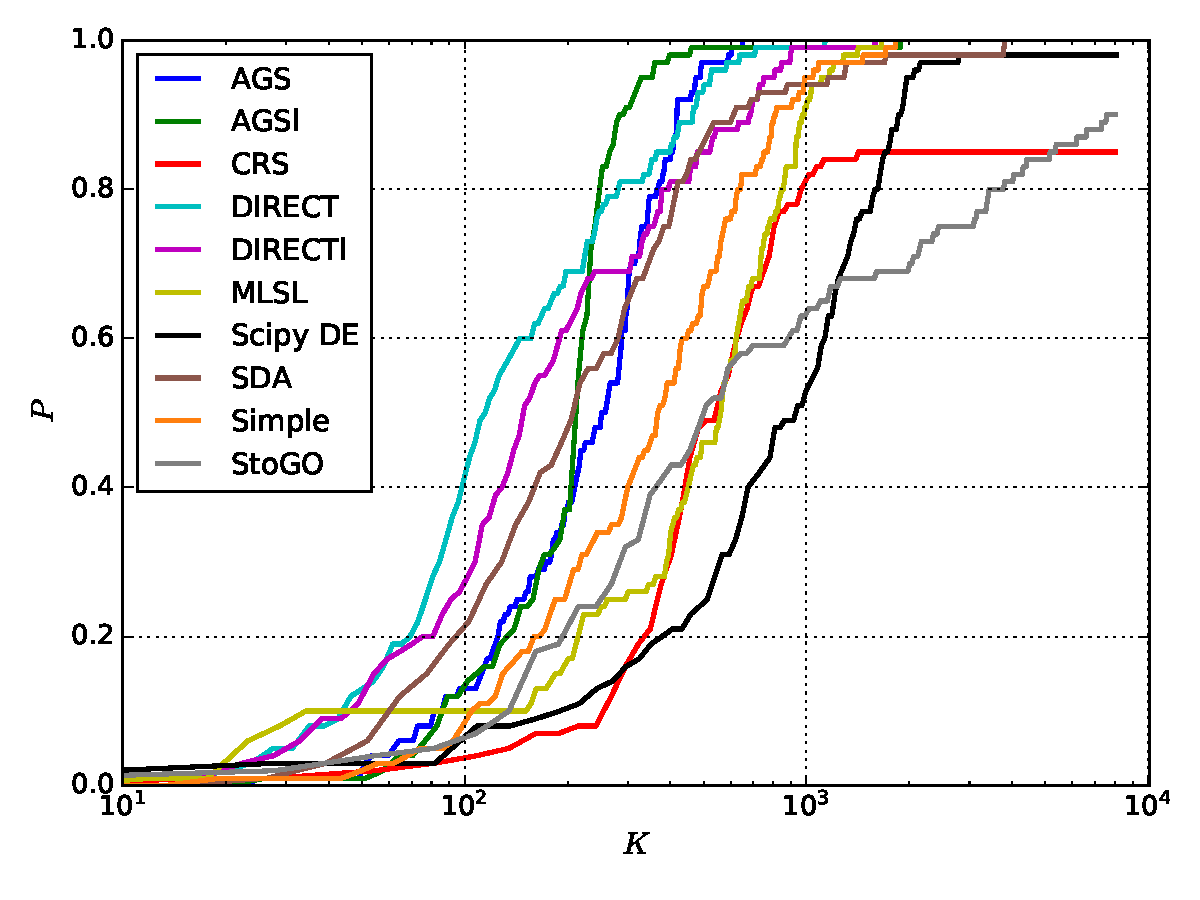
\includegraphics[width=0.95\textwidth]{../experiments/gklss2d/cmc.pdf}
  \caption{Class GKLS Simple 2d. $\Delta=2\cdot10^{-2}$}
\end{figure}

%table gklss2d
\begin{tabular}{lcc}
\hline
 Method   &  Average number of trials  &  Problems solved  \\
\hline
 AGS      &           254.89           &        100        \\
 AGSl     &           217.60           &        100        \\
 CRS      &           510.61           &        85         \\
 DIRECT   &           189.03           &        100        \\
 DIRECTl  &           255.21           &        100        \\
 MLSL     &           556.83           &        100        \\
 SDA      &           356.30           &        100        \\
 Scipy DE &           952.16           &        98         \\
 Simple   &           440.63           &        100        \\
 StoGO    &          1251.52           &        90         \\
\hline
\end{tabular}
\begin{figure}[H]
  \center
  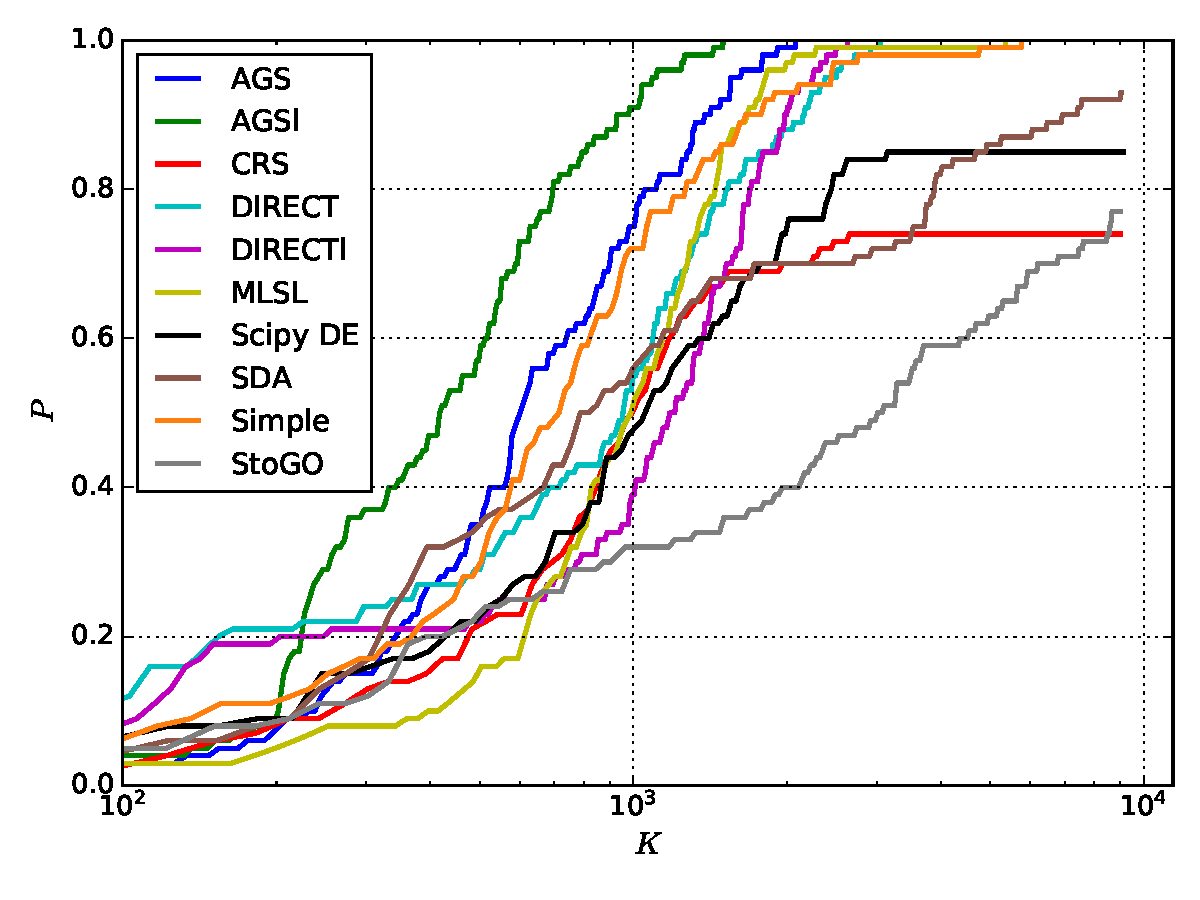
\includegraphics[width=0.95\textwidth]{../experiments/gklsh2d/cmc.pdf}
  \caption{Class GKLS Hard 2d. $\Delta=2\cdot10^{-2}$}
\end{figure}

%table gklsh2d
\begin{tabular}{lcc}
\hline
 Method   &  Average number of trials  &  Problems solved  \\
\hline
 AGS      &           728.71           &        100        \\
 AGSl     &           487.96           &        100        \\
 CRS      &           844.74           &        74         \\
 DIRECT   &           985.44           &        100        \\
 DIRECTl  &          1126.65           &        100        \\
 MLSL     &          1042.54           &        100        \\
 SDA      &          1637.92           &        93         \\
 Scipy DE &          1041.12           &        85         \\
 Simple   &           898.19           &        100        \\
 StoGO    &          2532.23           &        77         \\
\hline
\end{tabular}
\begin{figure}[H]
  \center
  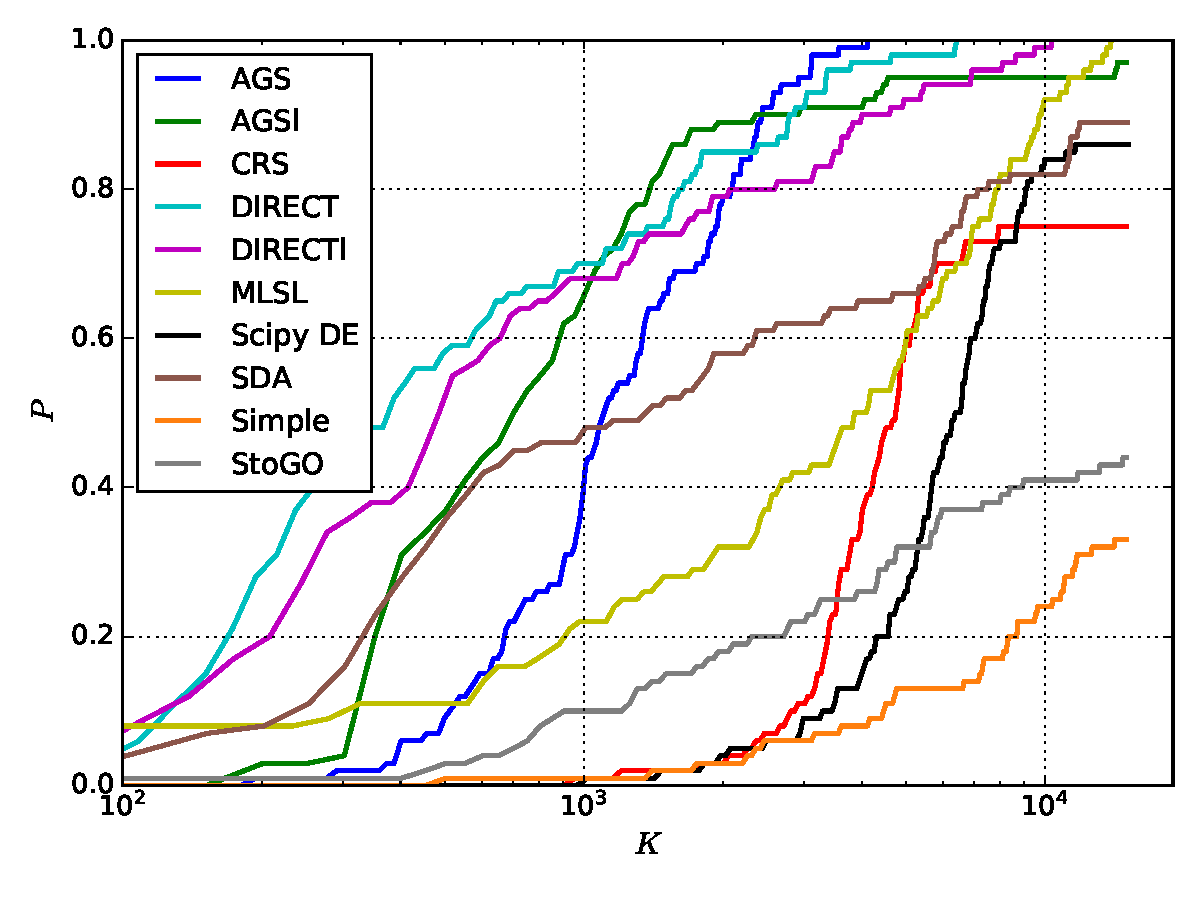
\includegraphics[width=0.95\textwidth]{../experiments/gklss3d/cmc.pdf}
  \caption{Class GKLS Simple 3d. $\Delta=2\cdot10^{-2}$}
\end{figure}

%table gklss3d
\begin{tabular}{lcc}
\hline
 Method   &  Average number of trials  &  Problems solved  \\
\hline
 AGS      &          1372.13           &        100        \\
 AGSl     &          1195.32           &        97         \\
 CRS      &          4145.81           &        75         \\
 DIRECT   &           973.64           &        100        \\
 DIRECTl  &          1477.79           &        100        \\
 MLSL     &          4609.17           &        100        \\
 SDA      &          2706.52           &        89         \\
 Scipy DE &          5956.94           &        86         \\
 Simple   &          7098.45           &        33         \\
 StoGO    &          3856.11           &        44         \\
\hline
\end{tabular}
\begin{figure}[H]
  \center
  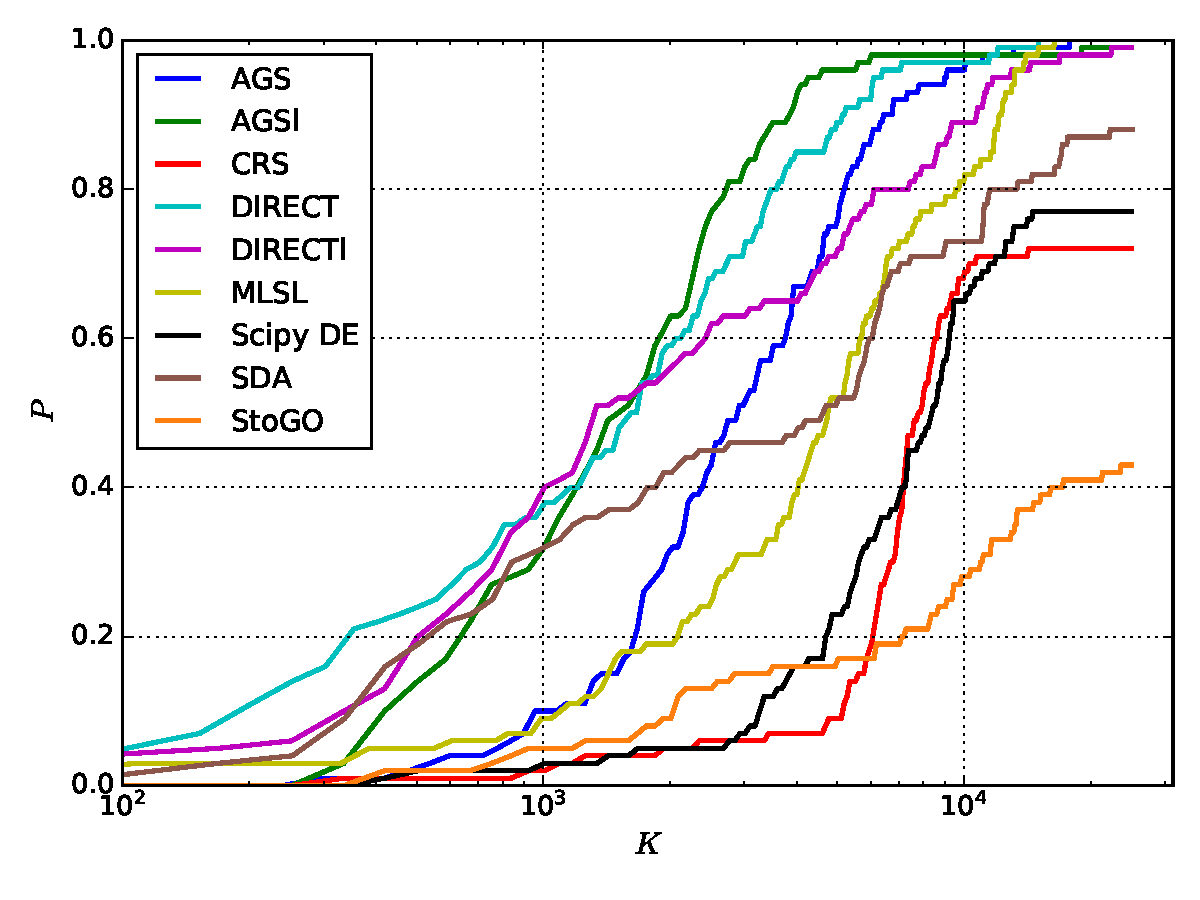
\includegraphics[width=0.95\textwidth]{../experiments/gklsh3d/cmc.pdf}
  \caption{Class GKLS Hard 3d. $\Delta=2\cdot10^{-2}$}
\end{figure}

%table gklsh3d
\begin{tabular}{lcc}
\hline
 Method   &  Average number of trials  &  Problems solved  \\
\hline
 AGS      &          3636.12           &        100        \\
 AGSl     &          1930.49           &        99         \\
 CRS      &          6786.96           &        72         \\
 DIRECT   &          2298.74           &        100        \\
 DIRECTl  &          3553.33           &        99         \\
 MLSL     &          5640.10           &        100        \\
 SDA      &          4708.43           &        88         \\
 Scipy DE &          6914.34           &        77         \\
 StoGO    &          7843.23           &        43         \\
\hline
\end{tabular}
\begin{figure}[H]
  \center
  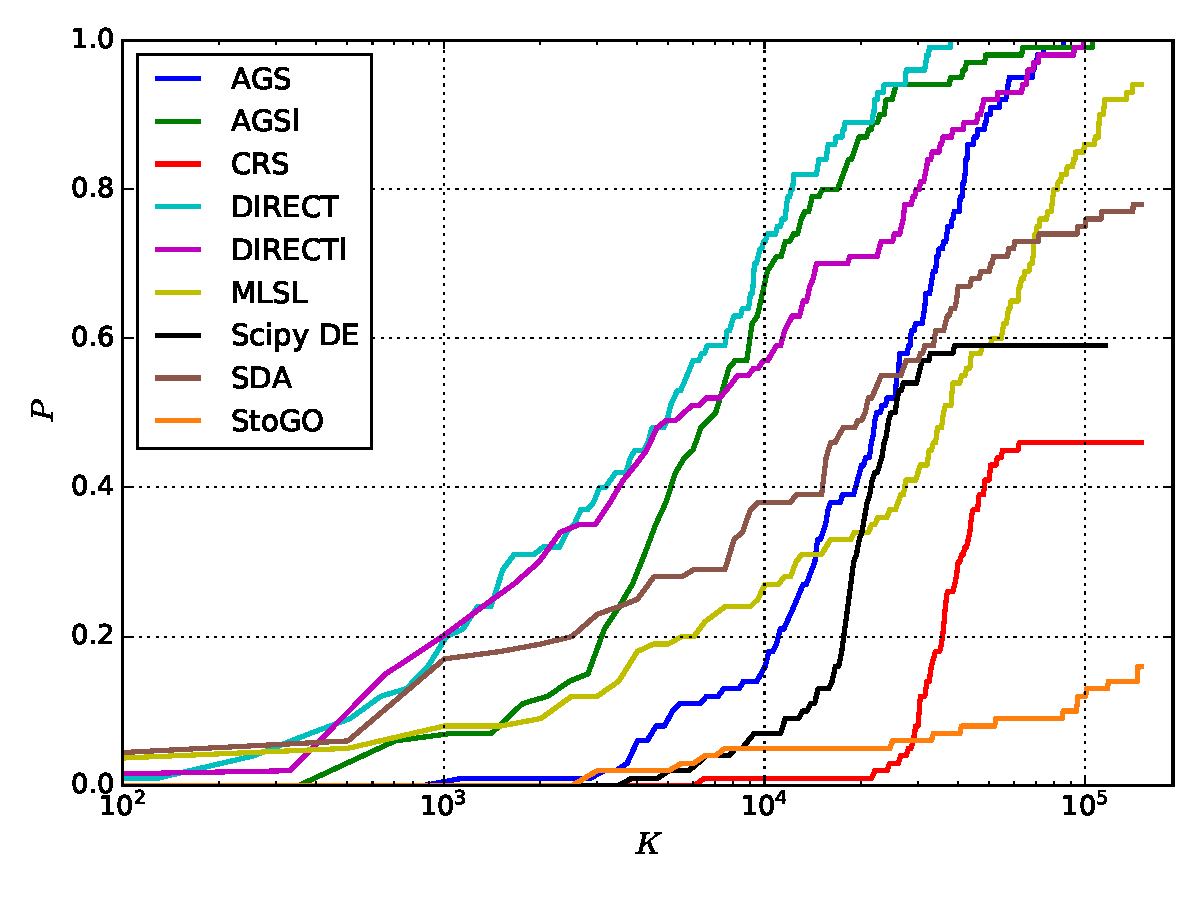
\includegraphics[width=0.95\textwidth]{../experiments/gklss4d/cmc.pdf}
  \caption{Class GKLS Simple 4d. $\Delta=2\cdot10^{-2}$}
\end{figure}

%table gklss4d
\begin{tabular}{lcc}
\hline
 Method   &  Average number of trials  &  Problems solved  \\
\hline
 AGS      &          26654.07          &        100        \\
 AGSl     &          11095.65          &        100        \\
 CRS      &          37436.76          &        46         \\
 DIRECT   &          7824.32           &        100        \\
 DIRECTl  &          15994.11          &        100        \\
 MLSL     &          41514.32          &        94         \\
 SDA      &          21417.90          &        78         \\
 Scipy DE &          19157.73          &        59         \\
 StoGO    &          59895.44          &        16         \\
\hline
\end{tabular}
\begin{figure}[H]
  \center
  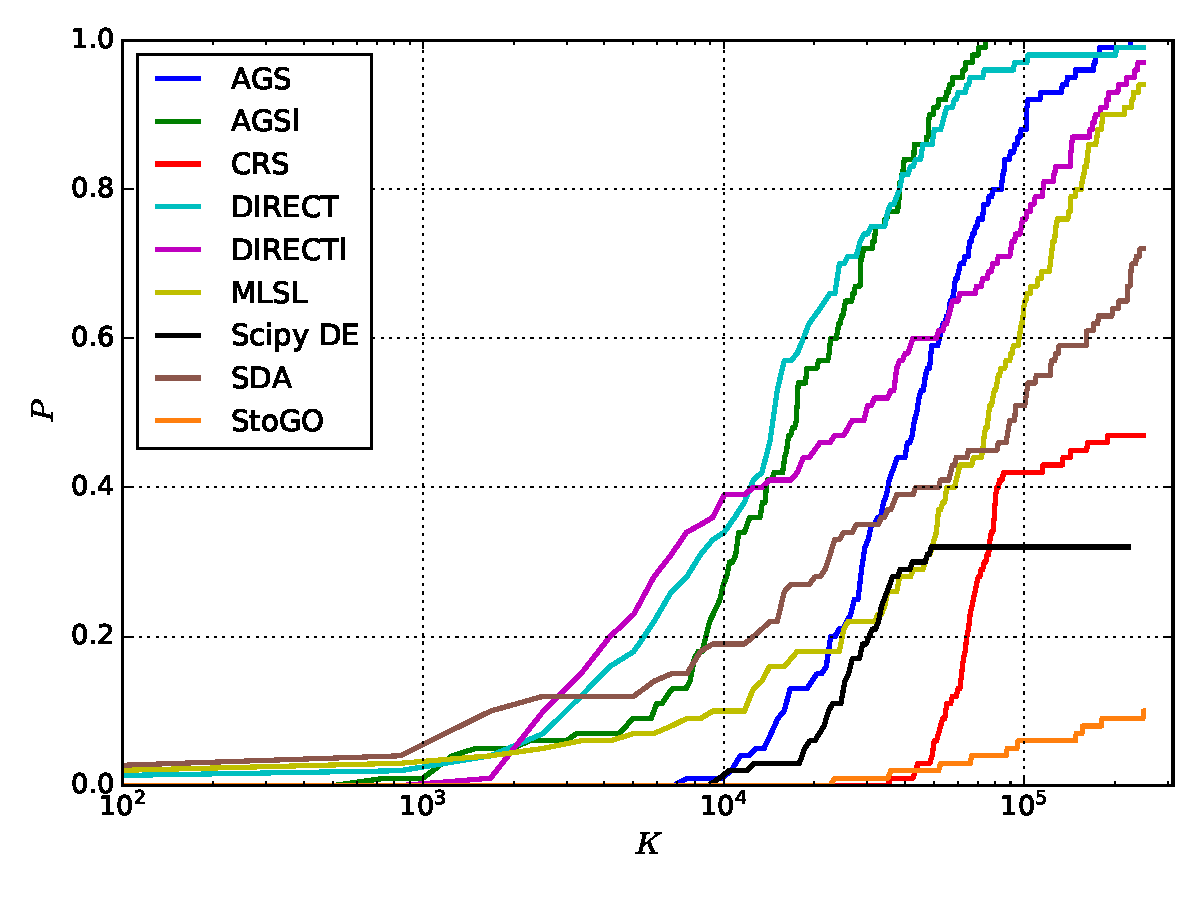
\includegraphics[width=0.95\textwidth]{../experiments/gklsh4d/cmc.pdf}
  \caption{Class GKLS Hard 4d. $\Delta=2\cdot10^{-2}$}
\end{figure}

%table gklsh4d
\begin{tabular}{lcc}
\hline
 Method   &  Average number of trials  &  Problems solved  \\
\hline
 AGS      &          54536.84          &        100        \\
 AGSl     &          23167.84          &        100        \\
 CRS      &          73779.32          &        47         \\
 DIRECT   &          23204.38          &        99         \\
 DIRECTl  &          54489.92          &        97         \\
 MLSL     &          80247.19          &        94         \\
 SDA      &          68815.53          &        72         \\
 Scipy DE &          27466.06          &        32         \\
 StoGO    &         109328.10          &        10         \\
\hline
\end{tabular}
\begin{figure}[H]
  \center
  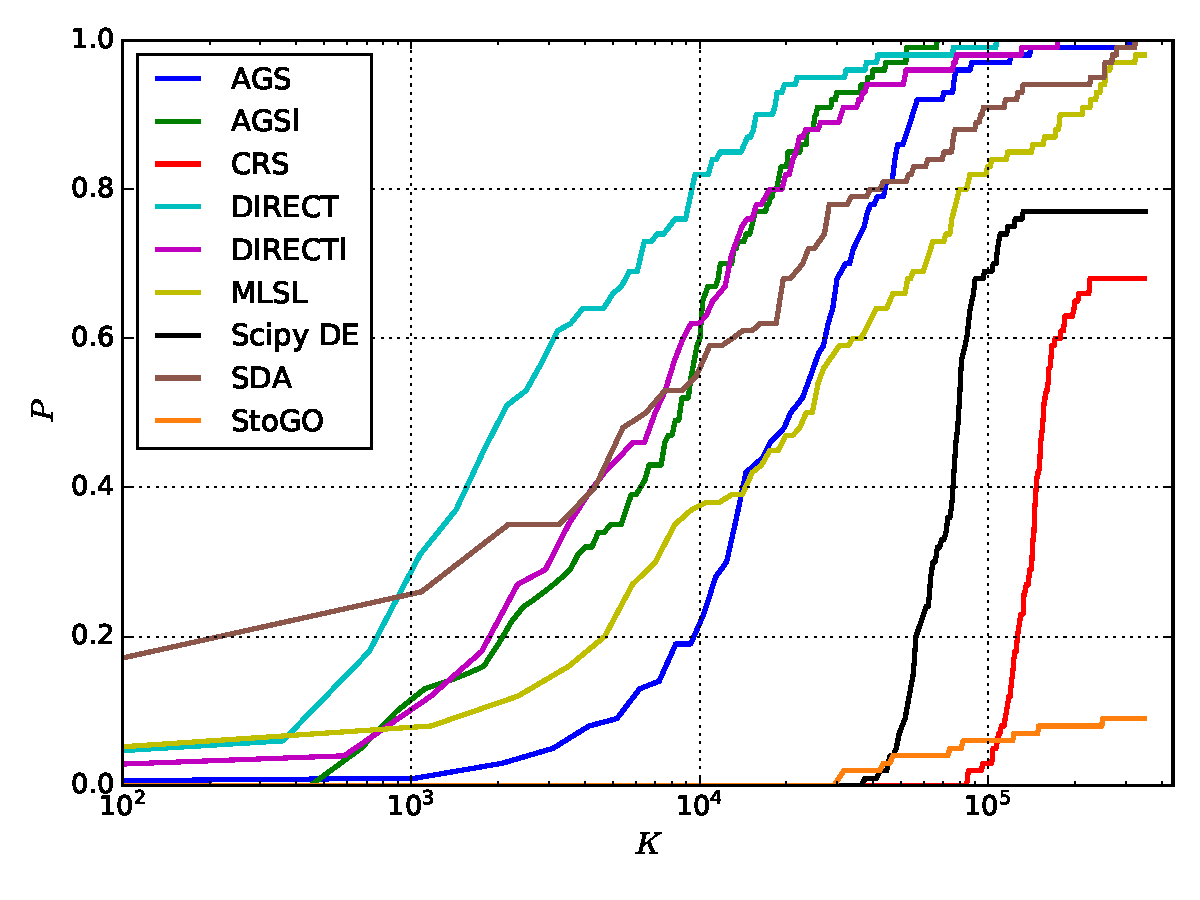
\includegraphics[width=0.95\textwidth]{../experiments/gklss5d/cmc.pdf}
  \caption{Class GKLS Simple 5d. $\Delta=2\cdot10^{-2}$}
\end{figure}

%table gklss5d
\begin{tabular}{lcc}
\hline
 Method   &  Average number of trials  &  Problems solved  \\
\hline
 AGS      &          29809.99          &        100        \\
 AGSl     &          11529.03          &        100        \\
 CRS      &         143574.99          &        68         \\
 DIRECT   &          7166.49           &        100        \\
 DIRECTl  &          13970.53          &        100        \\
 MLSL     &          52647.63          &        98         \\
 SDA      &          34255.31          &        100        \\
 Scipy DE &          73074.52          &        77         \\
 StoGO    &          91580.44          &         9         \\
\hline
\end{tabular}
\begin{figure}[H]
  \center
  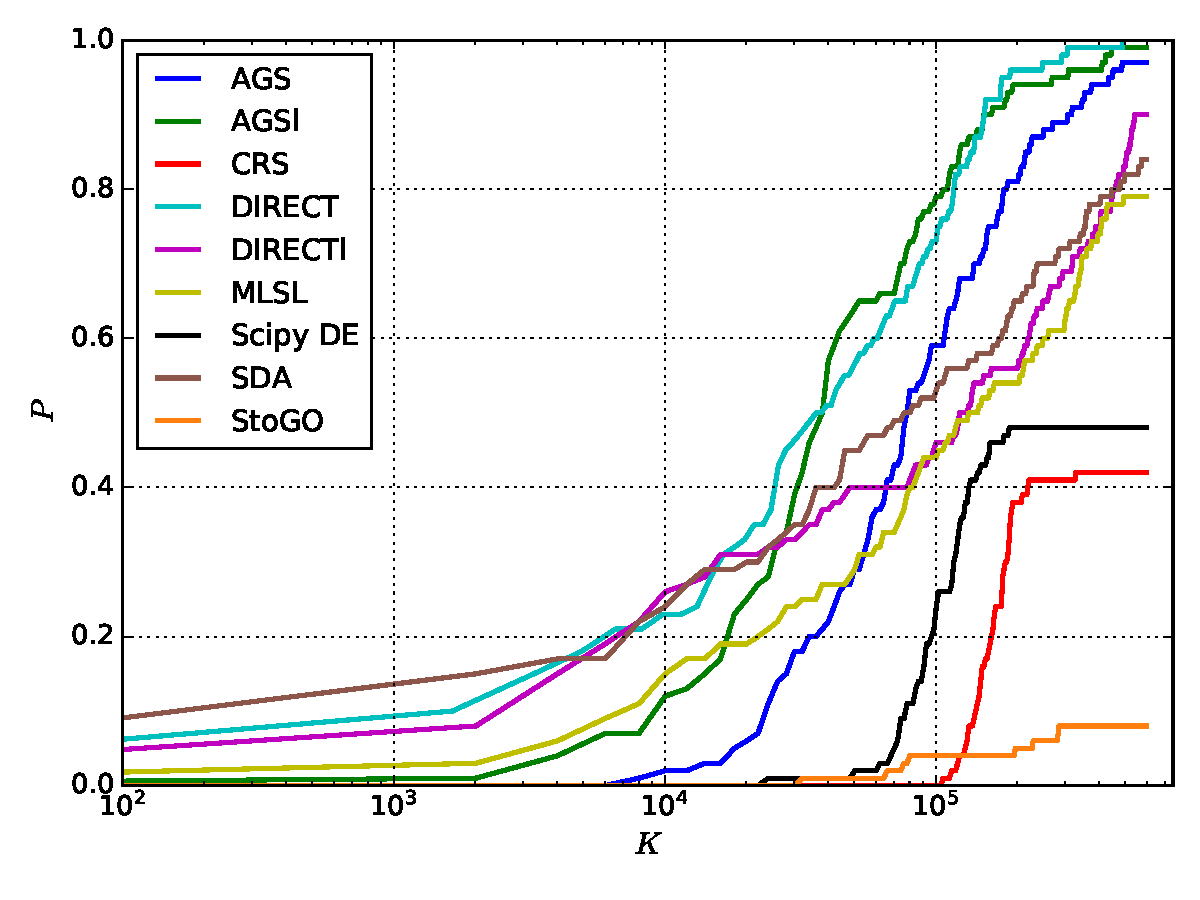
\includegraphics[width=0.95\textwidth]{../experiments/gklsh5d/cmc.pdf}
  \caption{Class GKLS Hard 5d. $\Delta=2\cdot10^{-2}$}
\end{figure}

%table gklsh5d
\begin{tabular}{lcc}
\hline
 Method   &  Average number of trials  &  Problems solved  \\
\hline
 AGS      &         113129.08          &        97         \\
 AGSl     &          67652.72          &        99         \\
 CRS      &         165192.76          &        42         \\
 DIRECT   &          66327.42          &        100        \\
 DIRECTl  &         164390.63          &        90         \\
 MLSL     &         138766.23          &        79         \\
 SDA      &         116973.10          &        84         \\
 Scipy DE &         105496.88          &        48         \\
 StoGO    &         155123.75          &         8         \\
\hline
\end{tabular}
\begin{figure}[H]
  \center
  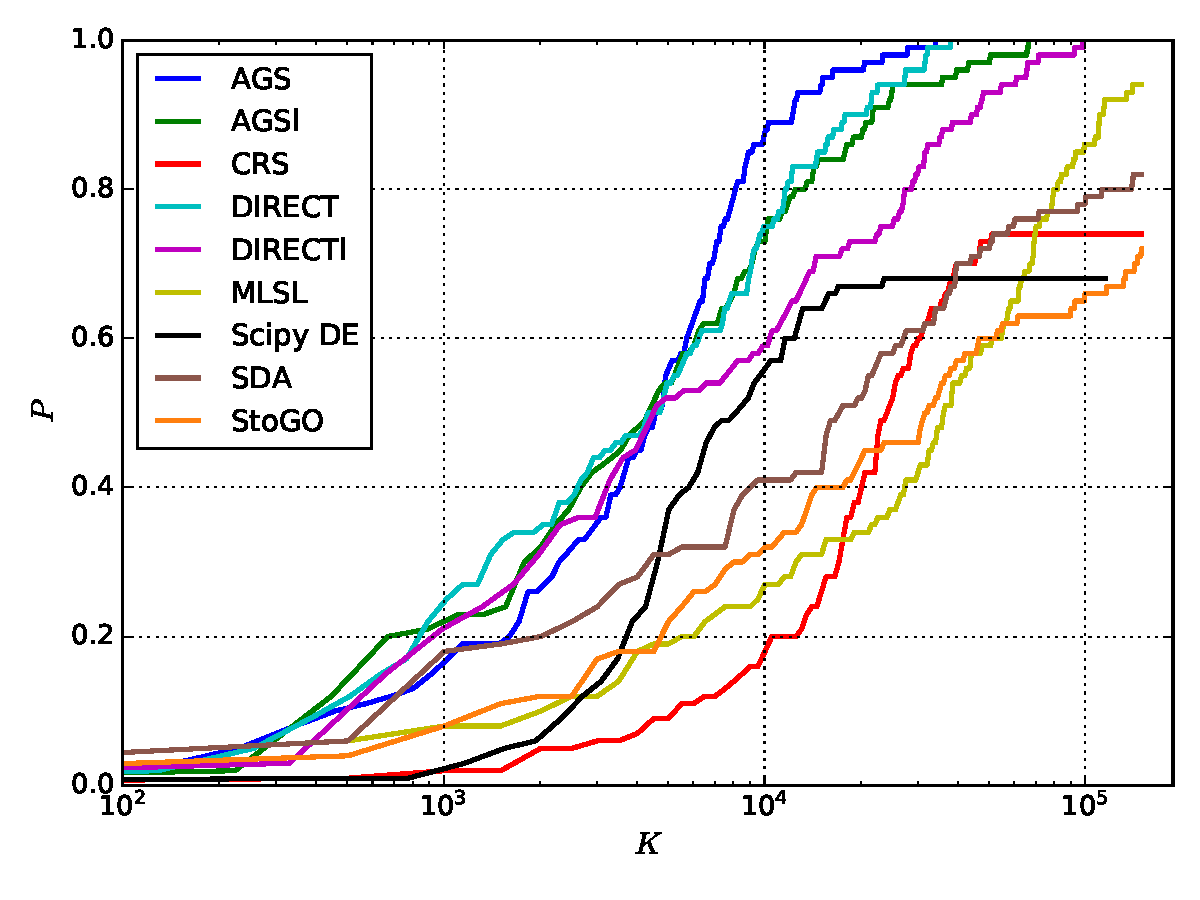
\includegraphics[width=0.95\textwidth]{../experiments/gklss4d_serg/cmc.pdf}
  \caption{Class GKLS Simple 4d. $\Delta=0.0632$}
\end{figure}

%table gklss4d_serg
\begin{tabular}{lcc}
\hline
 Method   &  Average number of trials  &  Problems solved  \\
\hline
 AGS      &          5729.82           &        100        \\
 AGSl     &          8847.40           &        100        \\
 CRS      &          19883.59          &        74         \\
 DIRECT   &          7328.78           &        100        \\
 DIRECTl  &          15010.01          &        100        \\
 MLSL     &          41484.80          &        94         \\
 SDA      &          22065.96          &        82         \\
 Scipy DE &          6271.24           &        68         \\
 StoGO    &          29359.22          &        72         \\
\hline
\end{tabular}
\begin{figure}[H]
  \center
  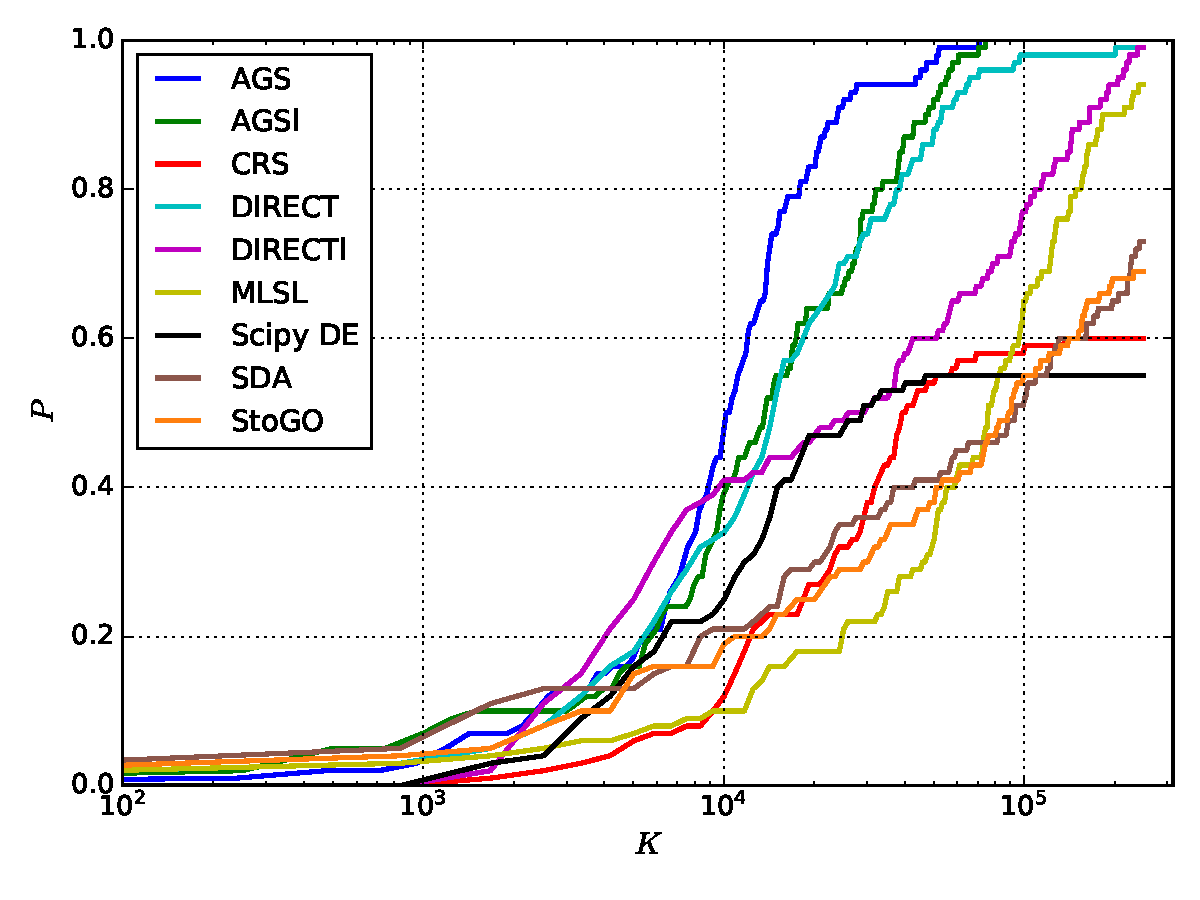
\includegraphics[width=0.95\textwidth]{../experiments/gklsh4d_serg/cmc.pdf}
  \caption{Class GKLS Hard 4d. $\Delta=0.0632$}

\end{figure}

%table gklsh4d_serg
\begin{tabular}{lcc}
\hline
 Method   &  Average number of trials  &  Problems solved  \\
\hline
 AGS      &          13113.40          &        100        \\
 AGSl     &          19826.36          &        100        \\
 CRS      &          27137.40          &        60         \\
 DIRECT   &          22884.35          &        99         \\
 DIRECTl  &          55596.07          &        99         \\
 MLSL     &          80220.11          &        94         \\
 SDA      &          68048.01          &        73         \\
 Scipy DE &          12487.64          &        55         \\
 StoGO    &          58925.54          &        69         \\
\hline
\end{tabular}
\begin{figure}[H]
  \center
  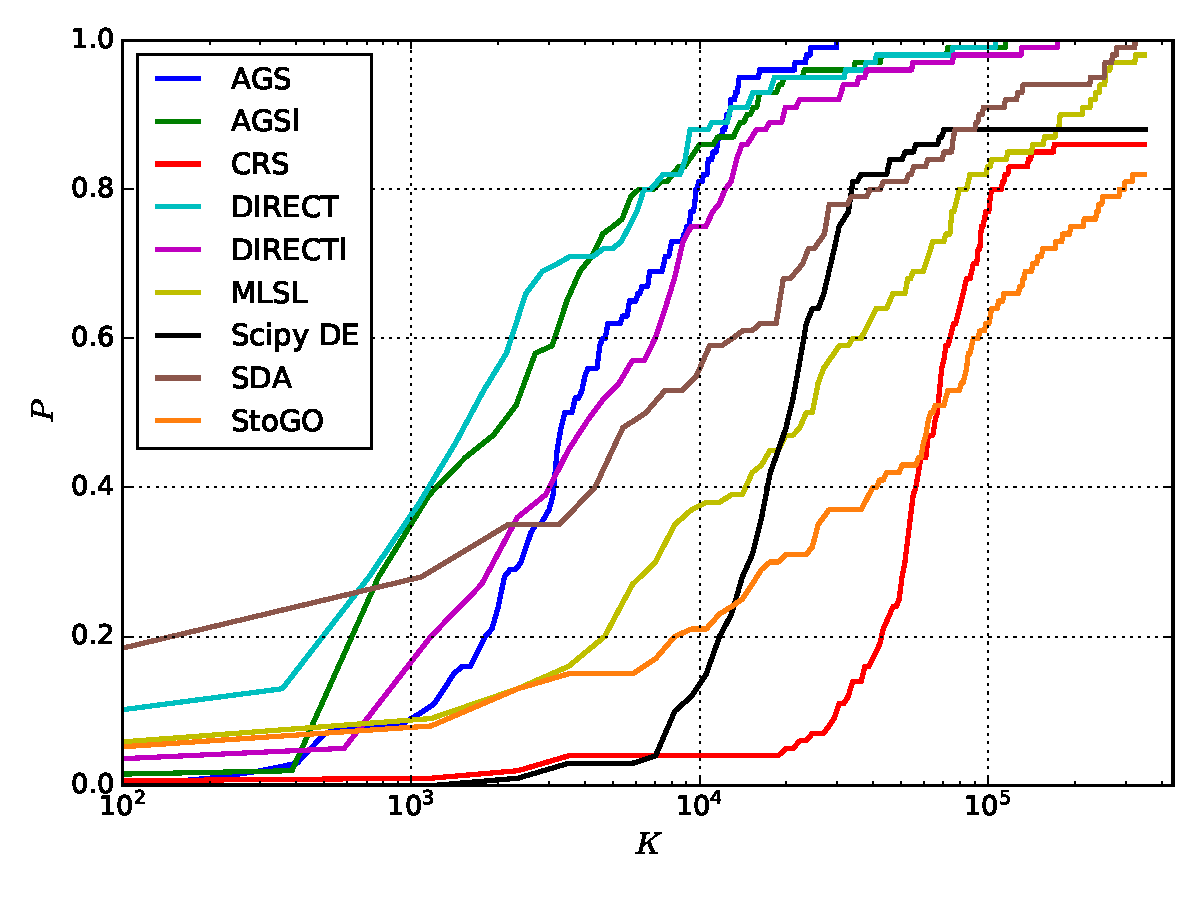
\includegraphics[width=0.95\textwidth]{../experiments/gklss5d_serg/cmc.pdf}
  \caption{Class GKLS Simple 5d. $\Delta=0.0796$}

\end{figure}

%table gklss5d_serg
\begin{tabular}{lcc}
\hline
 Method   &  Average number of trials  &  Problems solved  \\
\hline
 AGS      &          5821.47           &        100        \\
 AGSl     &          6314.25           &        100        \\
 CRS      &          62921.69          &        86         \\
 DIRECT   &          5966.13           &        100        \\
 DIRECTl  &          10795.46          &        100        \\
 MLSL     &          52609.18          &        98         \\
 SDA      &          34208.83          &        100        \\
 Scipy DE &          20859.38          &        88         \\
 StoGO    &          69206.76          &        82         \\
\hline
\end{tabular}
\begin{figure}[H]
  \center
  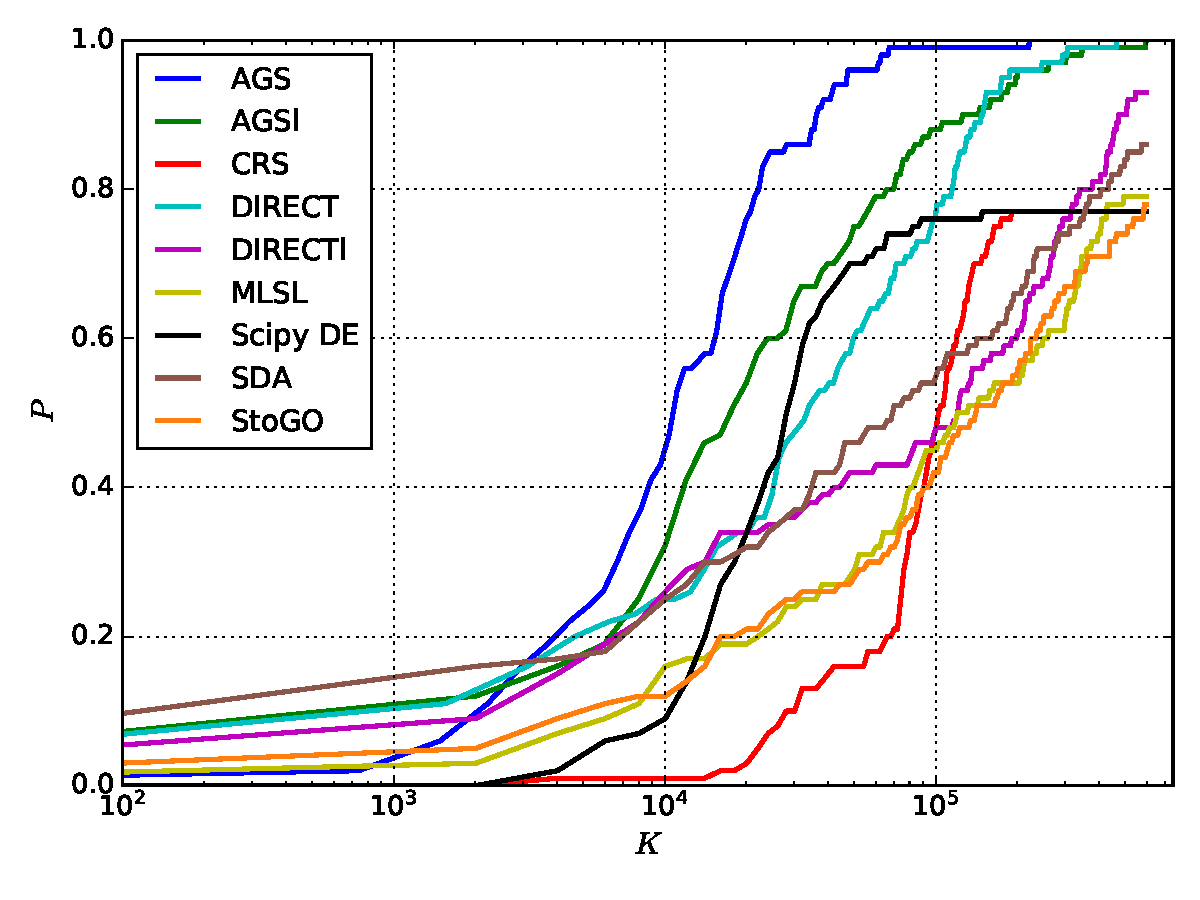
\includegraphics[width=0.95\textwidth]{../experiments/gklsh5d_serg/cmc.pdf}
  \caption{Class GKLS Hard 5d. $\Delta=0.0796$}

\end{figure}

%table gklsh5d_serg
\begin{tabular}{lcc}
\hline
 Method   &  Average number of trials  &  Problems solved  \\
\hline
 AGS      &          17008.61          &        100        \\
 AGSl     &          48514.29          &        100        \\
 CRS      &          87563.88          &        77         \\
 DIRECT   &          61657.32          &        100        \\
 DIRECTl  &         148637.82          &        93         \\
 MLSL     &         138011.78          &        79         \\
 SDA      &         115634.59          &        86         \\
 Scipy DE &          26850.04          &        77         \\
 StoGO    &         141886.49          &        78         \\
\hline
\end{tabular}
\end{document}
